\documentclass[11pt]{article}

% ----------------------------------------------------------------------
% Packages
% ----------------------------------------------------------------------
\usepackage[a4paper,margin=2.7cm]{geometry}
\usepackage[T1]{fontenc}
\usepackage[utf8]{inputenc}
\usepackage{lmodern}
\usepackage{amsmath,amssymb}
\usepackage{graphicx}
\usepackage[dvipsnames]{xcolor}
\usepackage{hyperref}
\usepackage[capitalise]{cleveref}
\usepackage{booktabs}
\usepackage{siunitx}
\usepackage[backend=biber,style=numeric,sorting=none]{biblatex}
\usepackage{setspace}
\addbibresource{references.bib}

\hypersetup{
    colorlinks=true,
    linkcolor=RoyalBlue,
    citecolor=RoyalBlue,
    urlcolor=RoyalBlue,
}

% ----------------------------------------------------------------------
% Macros
% ----------------------------------------------------------------------
\newcommand{\vS}{\boldsymbol{S}}
\newcommand{\SEP}{\boldsymbol{S}^{\mathrm{EP}}}
\newcommand{\chiEP}{\boldsymbol{\chi}^{\mathrm{EP}}}
\newcommand{\figplaceholder}[1]{\fbox{\parbox[c][#1][c]{0.85\linewidth}{\centering \textit{figure placeholder}}}}

% ----------------------------------------------------------------------
% Title block data
% ----------------------------------------------------------------------
\newcommand{\reporttitle}{Altermagnets and spin liquids}
\newcommand{\reportauthor}{Jonas Scheunemann}
\newcommand{\reportaffiliation}{University of Stuttgart}
\newcommand{\reportseminar}{Hauptseminar on Altermagnetism}
\newcommand{\reportsupervisors}{Supervised by Prof.\ Mathias Scheurer and MSc.\ Bernhard Putzer}
\newcommand{\reportdate}{June 1, 2026}

\begin{document}
\setstretch{1.125}

% ----------------------------------------------------------------------
% Title block (kept on the first page, no separate title page)
% ----------------------------------------------------------------------
\begin{center}
    {\LARGE\bfseries \reporttitle \par}
    \vspace{1.2em}
    {\large \reportauthor \par}
    \vspace{0.8em}
    {\normalsize \reportaffiliation \par}
    \vspace{0.6em}
    {\normalsize
        \reportseminar \\
        \reportsupervisors \par
    }
    \vspace{0.8em}
    {\normalsize \reportdate \par}
\end{center}

\vspace{1.5em}

% ----------------------------------------------------------------------
% Abstract
% ----------------------------------------------------------------------
\begin{center}
    {\bfseries Abstract}
\end{center}
\noindent
What happens to an altermagnet when quantum fluctuations destroy its spin
order? This report addresses this question following the work of Sobral,
Mandal, and Scheurer \cite{Sobral2025}.
Starting from a checkerboard $J_1$-$J_2$-$K$ Heisenberg model whose two
sublattices are related by a fourfold rotation instead of a translation, we
first map out the classical phase diagram. Besides collinear and nematic phases
it contains a noncoplanar orbital altermagnet, characterized by a staggered
pattern of scalar spin chiralities that is invariant under the combined
operation of time reversal and fourfold rotation. We then introduce quantum
spin liquids and the Schwinger boson construction, in which spins are
fractionalized into bosonic spinons subject to a local constraint. Every
classical phase possesses a neighboring spin liquid that inherits its discrete
symmetries. The neighbor of the orbital altermagnet is an altermagnetic
$\mathbb{Z}_2$ spin liquid: a phase without any spin order in which the
altermagnetic chirality pattern survives alongside topological order.

\vspace{2em}

% ----------------------------------------------------------------------
% Main text
% ----------------------------------------------------------------------
\section{Introduction}
\label{sec:intro}

Altermagnets have attracted a lot of attention in the last few years
\cite{Yuan2020,Smejkal2022,Smejkal2022a}. An altermagnet is a collinear magnet
whose total magnetization vanishes, but not for the reason familiar from
antiferromagnets. In a conventional antiferromagnet the two spin sublattices
are related by a lattice translation combined with time reversal $\Theta$, so
the moments cancel trivially. In an altermagnet the sublattices are instead
related by a point-group operation combined with time reversal, for example a
fourfold rotation $C_{4z}$ on the square lattice \cite{Smejkal2022}. The
consequences of this symmetry structure were the subject of the preceding talks
of this seminar: spin-split electronic bands despite zero net magnetization,
their observation in ARPES, magnon spectra, and nontrivial band topology.

All of this physics rests on one assumption: the spins form a long-range
ordered pattern, a static texture that breaks time reversal in a specific way.
In this report we go to the adjacent regime. We take an altermagnetic system
and make its frustrated couplings strong, so strong that quantum fluctuations
prevent the spins from ever settling into a static pattern. The spin order
melts, and the expectation value $\langle \hat{\vS}_i \rangle$ vanishes on
every site, even at zero temperature. The question is then: does anything
altermagnetic survive in a phase without spin order?

Following Sobral, Mandal, and Scheurer \cite{Sobral2025}, the answer is yes,
but the way it survives is subtle and requires new language. The altermagnetic
character does not live in the spin directions themselves but in
spin-rotation-invariant observables, specifically in a staggered pattern of
scalar spin chiralities. Describing the disordered phase requires the concepts
of quantum spin liquids, fractionalized excitations, and emergent gauge fields,
which we introduce along the way following the review by Savary and Balents
\cite{Savary2017}. The main result is a new phase of matter, the altermagnetic
$\mathbb{Z}_2$ spin liquid, which combines topological order with the symmetry
pattern of an altermagnet.

The question is not purely academic. Recent experiments indicate an interplay
between altermagnetism and magnetic frustration in Mn$_5$Si$_3$
\cite{Biniskos2022,Surgers2024} and in CsCr$_3$Sb$_5$ \cite{Xu2025}, so
frustrated altermagnets may well exist in real materials. The report is
organized as follows. \Cref{sec:model} introduces a minimal spin model that is
an altermagnet and can be strongly frustrated. \Cref{sec:classical} maps out
its classical phase diagram and introduces the observables that diagnose
altermagnetism without spin order. \Cref{sec:qsl} develops the Schwinger boson
description of quantum spin liquids, and \cref{sec:nearby} connects each
classical phase to its neighboring spin liquid and identifies the altermagnetic
spin liquid. Throughout we restrict ourselves to the insulating magnet; the
doped, itinerant case treated in Ref.~\cite{Sobral2025} is beyond the scope of
this report.

\section{The model}
\label{sec:model}

To make the question concrete we need a model that is an altermagnet and, at
the same time, can be strongly frustrated. Following Ref.~\cite{Sobral2025} we
consider a checkerboard Heisenberg magnet with two spin sublattices $A$ and $B$
per unit cell, placed on the bonds of a square lattice as sketched in
\cref{fig:model}. Denoting the spin operator on bond $i$ by $\hat{\vS}_i$, the
Hamiltonian reads
\begin{equation}
    \label{eq:model}
    H = J_1 \sum_{\langle i,j \rangle} \hat{\vS}_i \cdot \hat{\vS}_j
      + J_2 \sum_{\langle\langle i,j \rangle\rangle} \hat{\vS}_i \cdot \hat{\vS}_j
      + K \sum_{[i,j,k,l]} \left[ (\hat{\vS}_i \cdot \hat{\vS}_j)(\hat{\vS}_k \cdot \hat{\vS}_l)
      + (\hat{\vS}_i \cdot \hat{\vS}_l)(\hat{\vS}_k \cdot \hat{\vS}_j) \right].
\end{equation}
The first term is an antiferromagnetic nearest-neighbor exchange, $J_1 > 0$.
The second term couples next-nearest neighbors in the checkerboard pattern and
introduces frustration and competing orders. The ring-exchange term $K$ couples
any four spins on bonds sharing a common vertex in a way that preserves the
$C_{4v}$ point group, time reversal, spin rotation, and the Bravais lattice
translations. Its role is to lift degeneracies and stabilize additional phases;
in particular, it stabilizes the noncoplanar phase that will become central
later on.

\begin{figure}[t]
    \centering
    \begin{minipage}[c]{0.34\linewidth}
        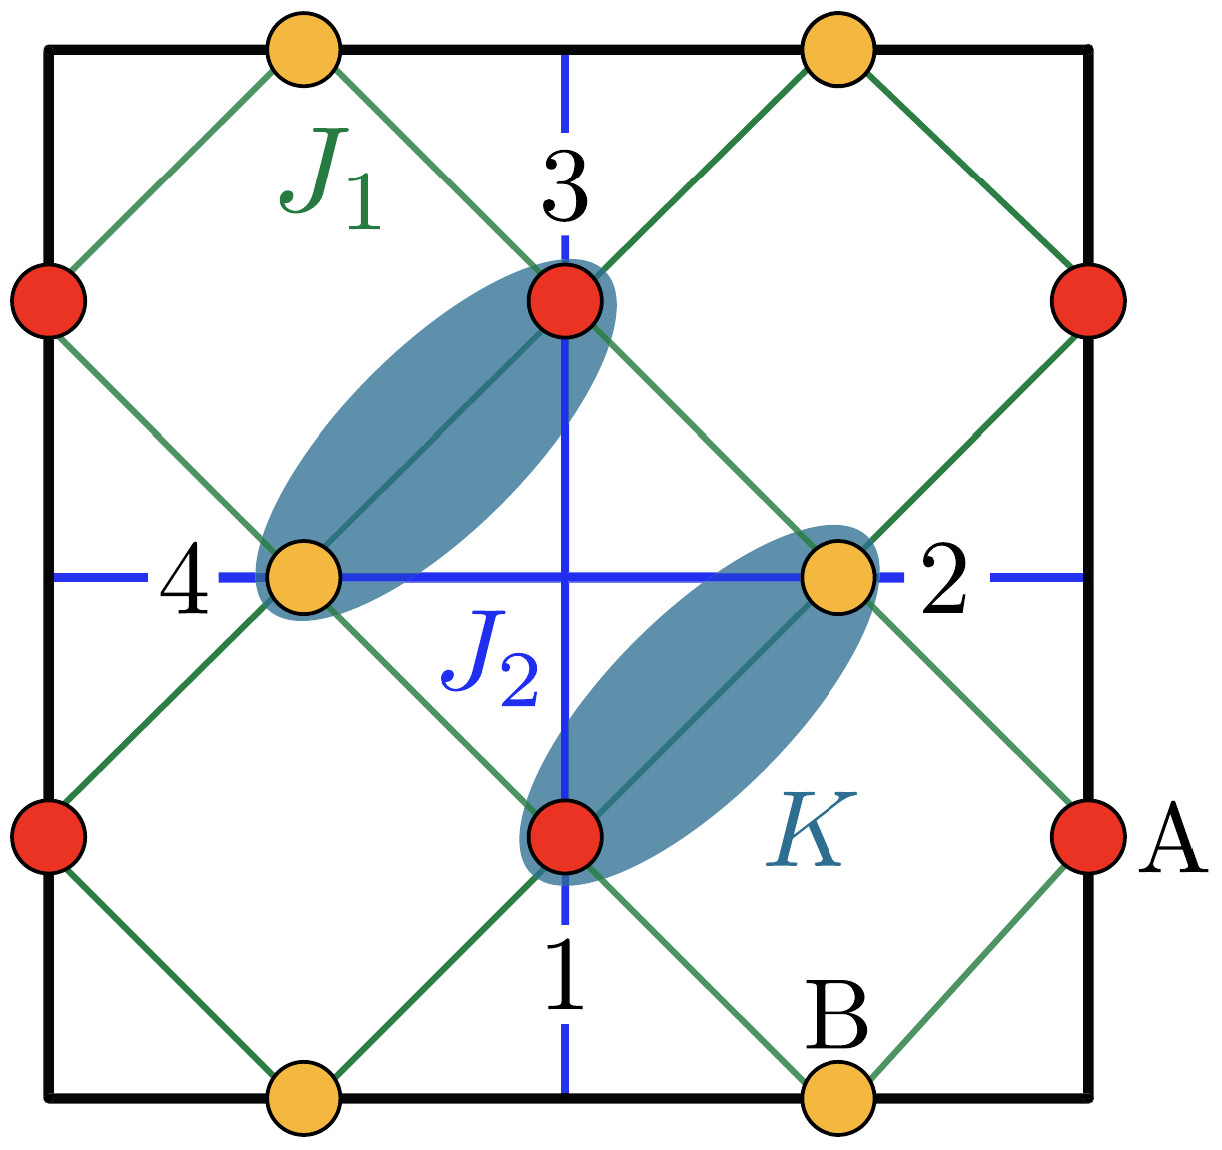
\includegraphics[width=\linewidth]{figures/checkerboard_model.png}
    \end{minipage}\hfill
    \begin{minipage}[c]{0.60\linewidth}
        \caption{The checkerboard model of \cref{eq:model}. The spins form two
        sublattices $A$ and $B$ on the bonds of a square lattice, related by the
        fourfold rotation $C_{4z}$ and not by a translation. Shown are the
        nearest-neighbor coupling $J_1$, the next-nearest-neighbor coupling $J_2$,
        and the ring-exchange term $K$. The sites $1$ to $4$ label the elementary
        plaquette used in \cref{eq:sep,eq:chiep}. Adapted from
        Ref.~\cite{Sobral2025}.}
        \label{fig:model}
    \end{minipage}
\end{figure}

The decisive property of the model is its symmetry. With only $J_1$ the model
is identical to a square-lattice antiferromagnet rotated by $45^\circ$; in that
case an artificial translation symmetry connects the two sublattices, and the
ground state would be a conventional antiferromagnet. Finite $J_2$ and $K$
break this translation. What remains is the fourfold rotation $C_{4z}$ that
maps $A$ onto $B$, and this is exactly the altermagnetic symmetry: the total
magnetization is forced to vanish by a rotation instead of a translation. We
stress that the following analysis is not limited to this particular model; it
is simply a minimal explicit example in which all steps can be carried out.

\section{Classical phase diagram}
\label{sec:classical}

\subsection{Classical spin ansatz}
\label{sec:ansatz}

We first analyze the magnetic phases of \cref{eq:model} in the classical limit
$S \to \infty$, where the spins become classical vectors and quantum
fluctuations are absent. For the direction of the magnetization on sublattice
$\mu = A, B$ in the unit cell at position $\boldsymbol{R}$ we make the general
spiral ansatz
\begin{equation}
    \label{eq:ansatz}
    \vS_\mu(\boldsymbol{R}) \propto
    \hat{\boldsymbol{a}} \cos(\boldsymbol{Q} \cdot \boldsymbol{R} - \varphi_\mu)
    + \hat{\boldsymbol{b}} \sin(\boldsymbol{Q} \cdot \boldsymbol{R} - \varphi_\mu)
    + \hat{\boldsymbol{c}}\, \eta_\mu,
\end{equation}
where $\hat{\boldsymbol{a}}$, $\hat{\boldsymbol{b}}$, and
$\hat{\boldsymbol{c}}$ are three arbitrary orthonormal vectors. The ordering
wavevector $\boldsymbol{Q}$ sets the period and direction of the spiral, the
phase $\varphi_\mu$ fixes the relative angle between the two sublattices, and
$\eta_\mu$ is an out-of-plane canting that vanishes for all coplanar textures.
Without loss of generality one sets $\varphi_A = 0$ and $\varphi_B \equiv
\varphi$. For every point of the $(J_2, K)$ plane the classical energy is then
minimized over the parameters $\{Q_x, Q_y, \varphi, \eta_A, \eta_B\}$, in
practice by a grid search followed by gradient descent \cite{Sobral2025}. The
resulting phase diagram is shown in \cref{fig:phasediagram} and the
corresponding spin textures in \cref{fig:spin_textures}.

\begin{figure}[ht]
    \centering
    \begin{minipage}[c]{0.4\linewidth}
        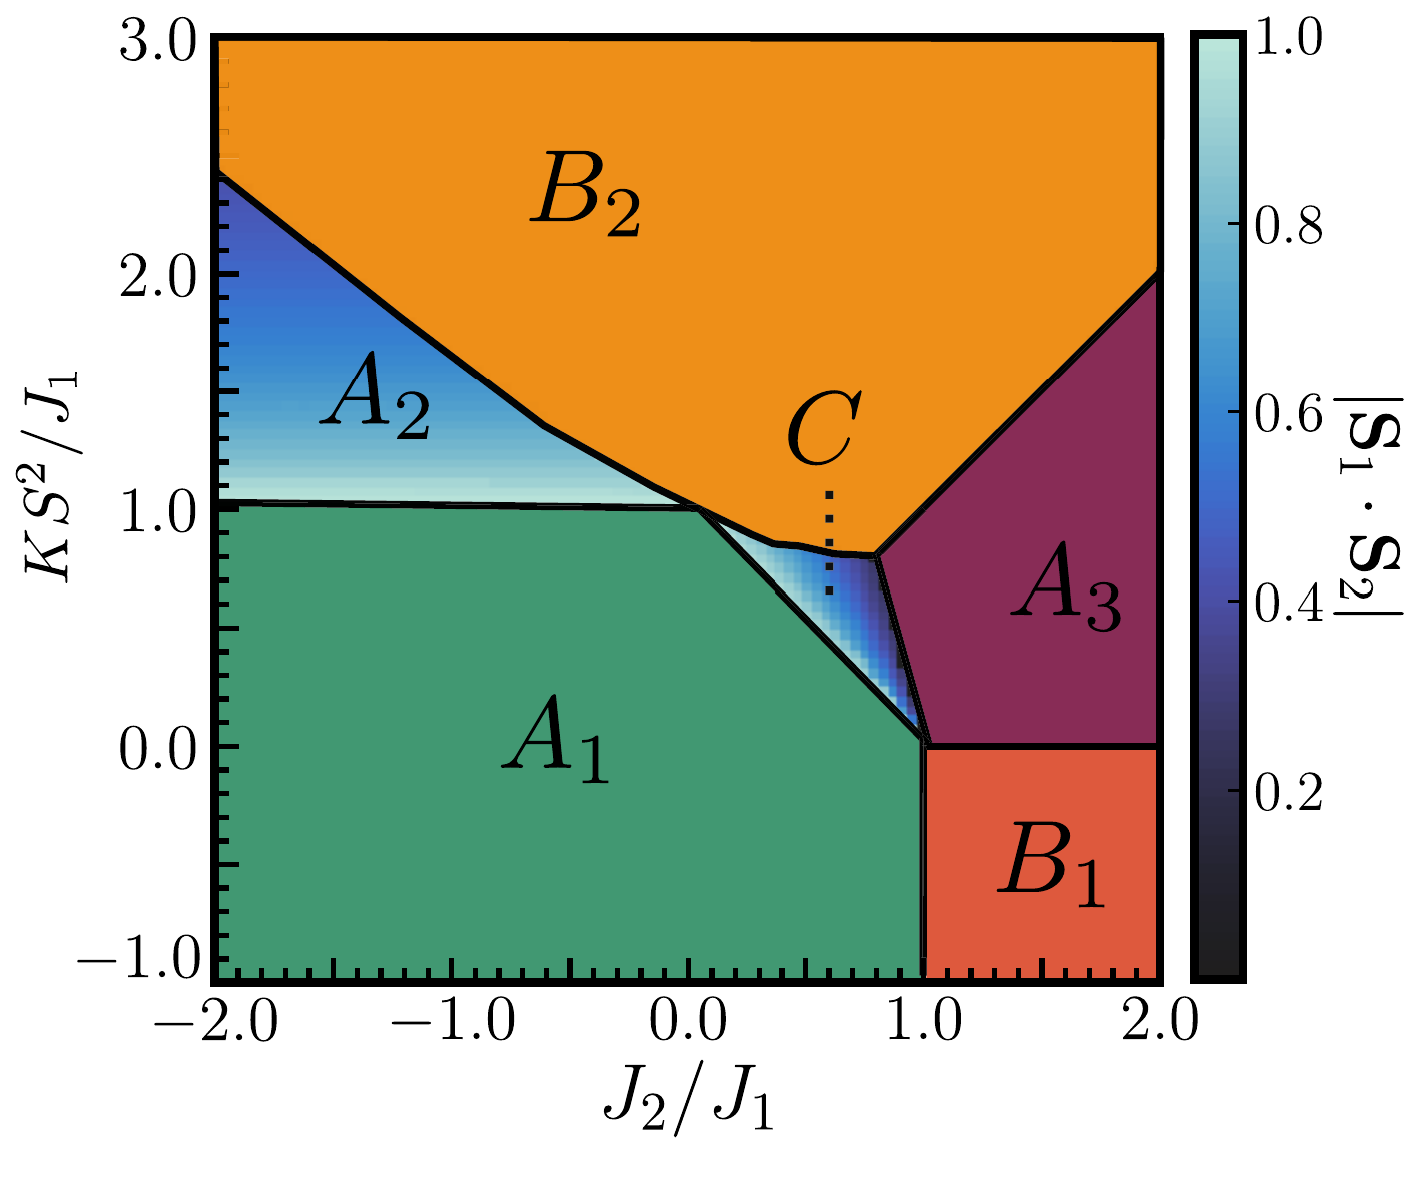
\includegraphics[width=\linewidth]{figures/classical_phase_diagram}
    \end{minipage}\hfill
    \begin{minipage}[c]{0.60\linewidth}
        \caption{Classical phase diagram of the model in the $(J_2, K)$ plane,
        obtained by minimizing the energy of the Ansatz \eqref{eq:ansatz}.}
        \label{fig:phasediagram}
    \end{minipage}
\end{figure}

\subsection{Spin-rotation-invariant observables}
\label{sec:observables}

Before walking through the phases we introduce the observables that will carry
the story. The reason is the following: when we later melt the ordered phases
into spin liquids, spin-rotation invariance is restored and $\langle
\hat{\vS}_i \rangle = 0$ on every site. Any conventional magnetic order
parameter then vanishes identically. If we want to track symmetries into the
disordered regime, we need quantities that are invariant under global spin
rotations and can therefore remain nonzero even when there is no spin
polarization.

Both observables are defined on an elementary plaquette (EP) of four spins,
labeled $1$ to $4$ as in \cref{fig:model}. The first is the vector of
nearest-neighbor scalar products,
\begin{equation}
    \label{eq:sep}
    \SEP = \left( \vS_1 \cdot \vS_2,\; \vS_2 \cdot \vS_3,\;
    \vS_3 \cdot \vS_4,\; \vS_4 \cdot \vS_1 \right)^T.
\end{equation}
It is manifestly invariant under global spin rotations. If all four components
are equal, the fourfold rotation $C_{4z}$ is preserved; if they differ around
the plaquette, $C_{4z}$ is broken. $\SEP$ is therefore the nematicity detector
in the spin-rotation-invariant sector. The second observable is the vector of
scalar spin chiralities,
\begin{equation}
    \label{eq:chiep}
    \chiEP = \left( \vS_1 \cdot (\vS_2 \times \vS_3),\;
    \vS_2 \cdot (\vS_3 \times \vS_4),\;
    \vS_3 \cdot (\vS_4 \times \vS_1),\;
    \vS_4 \cdot (\vS_1 \times \vS_2) \right)^T.
\end{equation}
A scalar spin chirality requires three noncoplanar spins; it vanishes
identically for every coplanar texture. Under time reversal all spins flip
sign, and a triple product of three flipped vectors acquires a minus sign, so
$\chiEP$ is odd under $\Theta$. It is the time-reversal detector in the
spin-rotation-invariant sector. Together the two observables tell us whether
$C_{4z}$ and $\Theta$ are broken and, more importantly, how they are broken.

\begin{figure}[ht]
    \centering
    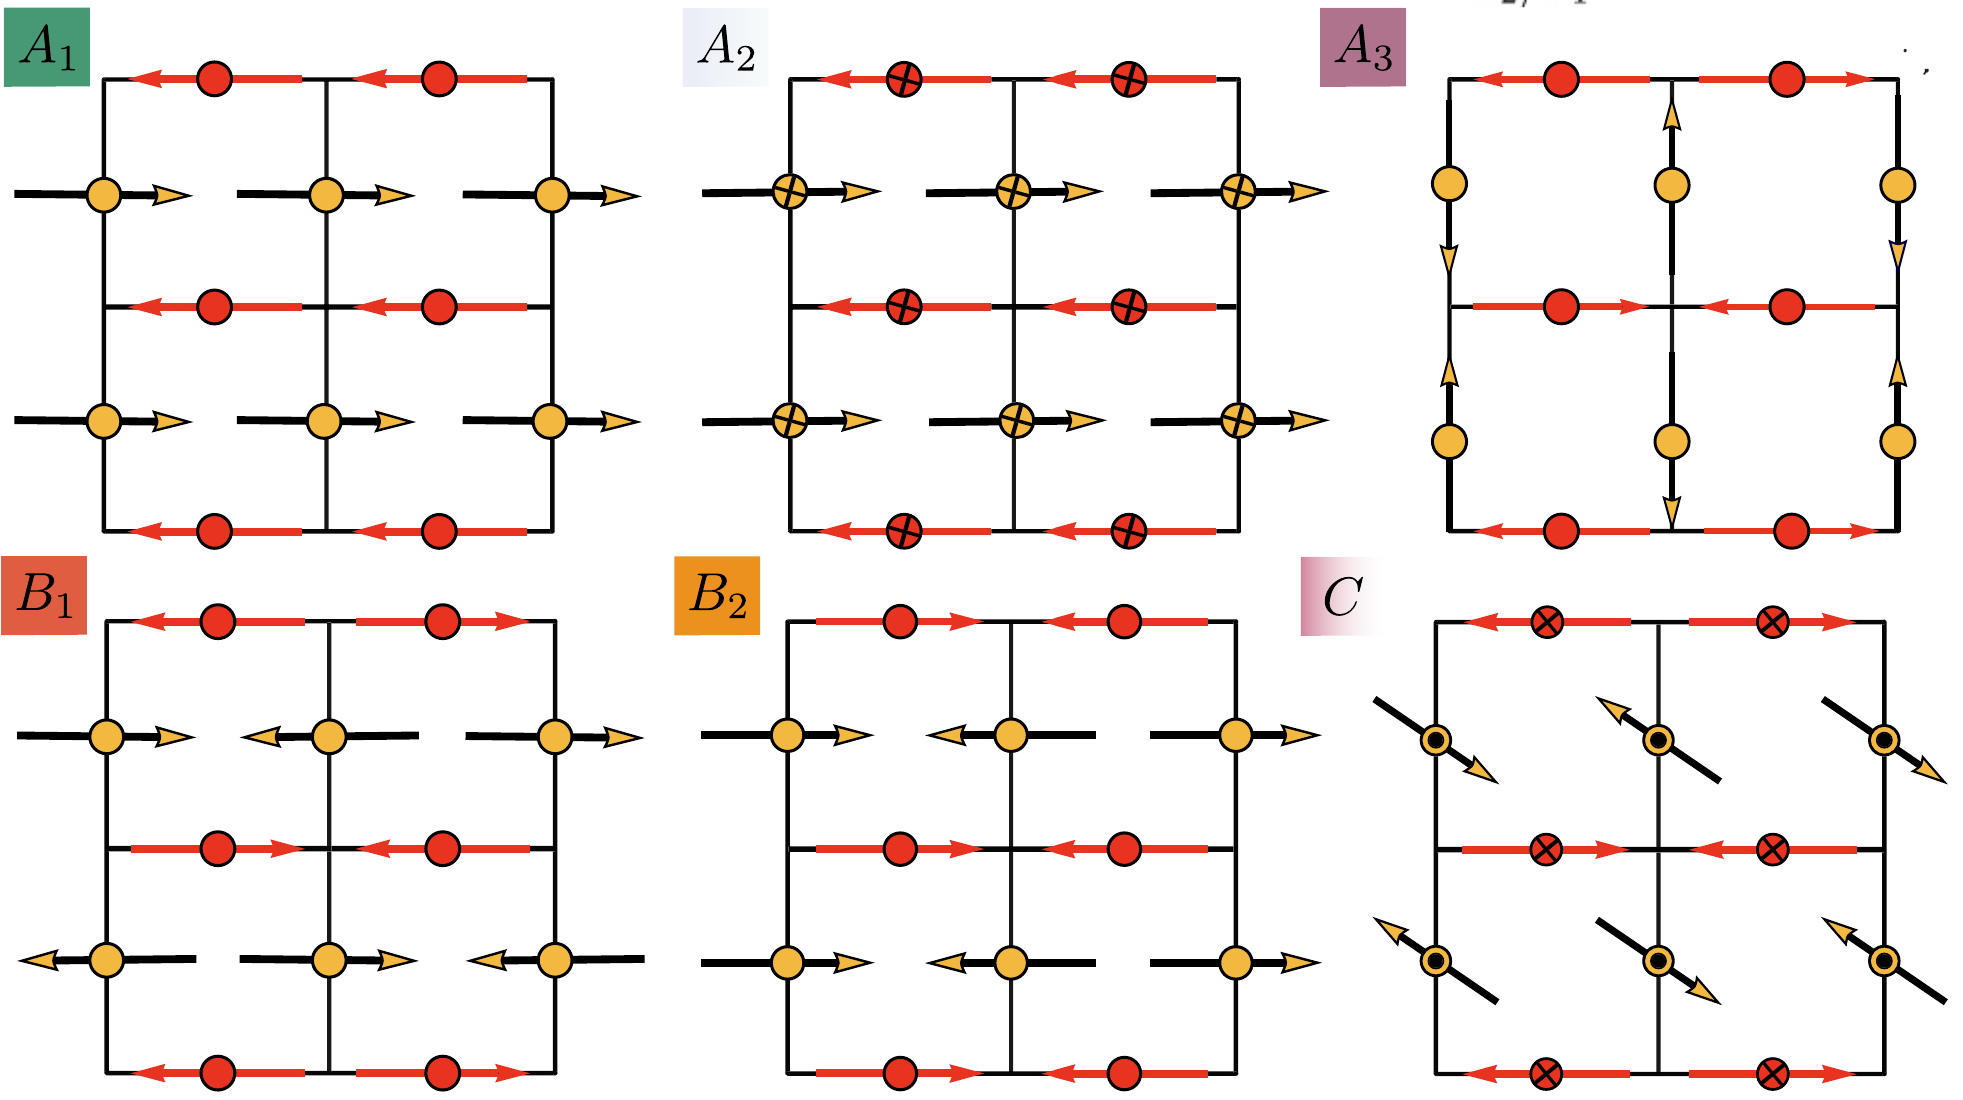
\includegraphics[width=0.8\linewidth]{figures/classical_spin_textures}
    \caption{Classical spin textures for the six phases listed in \cref{tab:phases}. We can 
    distinguish collinear, coplanar, and noncoplanar textures, 
    as well as the presence or absence of a net magnetization. Adapted from Ref.~\cite{Sobral2025}.}
    \label{fig:spin_textures}
\end{figure}

\subsection{The magnetic phases}
\label{sec:phases}

\Cref{tab:phases} summarizes the six phases of the classical phase diagram
together with their observables and symmetries; the last column already lists
the gauge structure of the associated spin liquids that we construct in
\cref{sec:nearby}.

\begin{table}[t]
    \centering
    \caption{Summary of the classical magnetic phases of \cref{eq:model} and
    their spin-rotation-invariant observables, following
    Ref.~\cite{Sobral2025}. Here $s_0, s_0', \xi_0 > 0$ are nonuniversal
    numbers that depend on the couplings, $M$ denotes the total magnetization,
    and the listed symmetries are those of spin-rotation-invariant observables.
    The last column gives the invariant gauge group (IGG) of the associated
    spin liquid of \cref{sec:nearby}.}
    \label{tab:phases}
    \vspace{0.5em}
    \small
    \begin{tabular}{llccccc}
        \toprule
        Label & Type & $\SEP$ & $\chiEP$ & $M$ & Symmetries & IGG \\
        \midrule
        $A_1$ & collinear altermagnet & $-(1,1,1,1)$ & $0$ & $0$ & $C_{4z}, \sigma_v, \Theta$ & U(1) \\
        $A_2$ & canted altermagnet & $-(s_0,s_0,s_0,s_0)$ & $0$ & $\neq 0$ & $C_{4z}, \sigma_v, \Theta$ & $\mathbb{Z}_2$ \\
        $A_3$ & orthogonal antiferromagnet & $(0,0,0,0)$ & $0$ & $0$ & $C_{4z}, \sigma_v, \Theta$ & $\mathbb{Z}_2$ \\
        $B_1$ & collinear nematic & $(-1,1,-1,1)$ & $0$ & $0$ & $C_{2z}, \sigma_d, \Theta$ & U(1) \\
        $B_2$ & collinear odd parity & $(1,1,-1,-1)$ & $0$ & $0$ & $\sigma_v, \Theta$ & U(1) \\
        $C$ & orbital altermagnet & $-(s_0',s_0',s_0',s_0')$ & $(-\xi_0,\xi_0,-\xi_0,\xi_0)$ & $0$ & $C_{4z}\Theta, \sigma_v$ & $\mathbb{Z}_2$ \\
        \bottomrule
    \end{tabular}
\end{table}

The anchor of the story is the collinear altermagnet $A_1$, stabilized at small
$J_2$ and $K$. All spins on sublattice $A$ point in one direction and all spins
on $B$ in the opposite direction. Every nearest-neighbor bond then carries the
same antiferromagnetic spin product, $\SEP = -(1,1,1,1)$, so $C_{4z}$ is
intact, and since the texture is collinear the chirality vanishes. Modulo
global spin rotations, all magnetic point-group symmetries are preserved. The
total magnetization vanishes, and it does so because of $C_{4z}$, not because
of a translation: $A_1$ is a collinear altermagnet.

Increasing $K$ leads to a second-order transition into the canted altermagnet
$A_2$. Both sublattices develop the same out-of-plane tilt, which produces a
finite magnetization $M \neq 0$. In the spin-rotation-invariant sector nothing
changes: $\SEP$ stays uniform, only with reduced magnitude, and the chirality
stays zero. At large $J_2$ one finds the orthogonal antiferromagnet $A_3$, a
spiral with $\boldsymbol{Q} = (\pi, \pi)$ and $\varphi = \pi/2$ in which
neighboring spins are perpendicular. All nearest-neighbor products vanish,
$\SEP = (0,0,0,0)$, and the state can be viewed as an antiferromagnet with four
spins in an enlarged unit cell. Like $A_1$ and $A_2$ it preserves all
symmetries modulo spin rotations.

The phase diagram further contains two nematic phases. In $B_1$, reached from
$A_3$ by a first-order transition when the sign of $K$ is reversed, horizontal
bonds carry antiparallel spins while vertical bonds carry nearly parallel
spins. The spin products alternate around the plaquette, $\SEP = (-1,1,-1,1)$,
and $C_{4z}$ is broken down to a twofold rotation. In $B_2$, stabilized when
$K > 0$ dominates the energetics, the components instead group pairwise, $\SEP
= (1,1,-1,-1)$, which is a different breaking pattern of the same rotational
symmetry. Both nematic phases remain coplanar, so $\chiEP = 0$ and time
reversal is preserved in spin-rotation-invariant observables.

The most frustrated region of the phase diagram hosts the key phase of this
report: the noncoplanar phase $C$. Here the two sublattices cant out of the
plane in opposite directions, $\eta_A = -\eta_B$. The spin products $\SEP$
remain uniform, so phase $C$ is not nematic. The new feature is the chirality.
Because the texture is noncoplanar, the scalar spin chiralities are nonzero,
and their pattern around the plaquette is staggered,
\begin{equation}
    \label{eq:chipattern}
    \chiEP \propto (-1, 1, -1, 1).
\end{equation}
As shown in \cref{fig:classical_transitions}(a,b), phase $C$ is reached from $A_1$ by a
second-order transition at which this chirality grows continuously from zero.

\begin{figure}[ht]
    \centering
    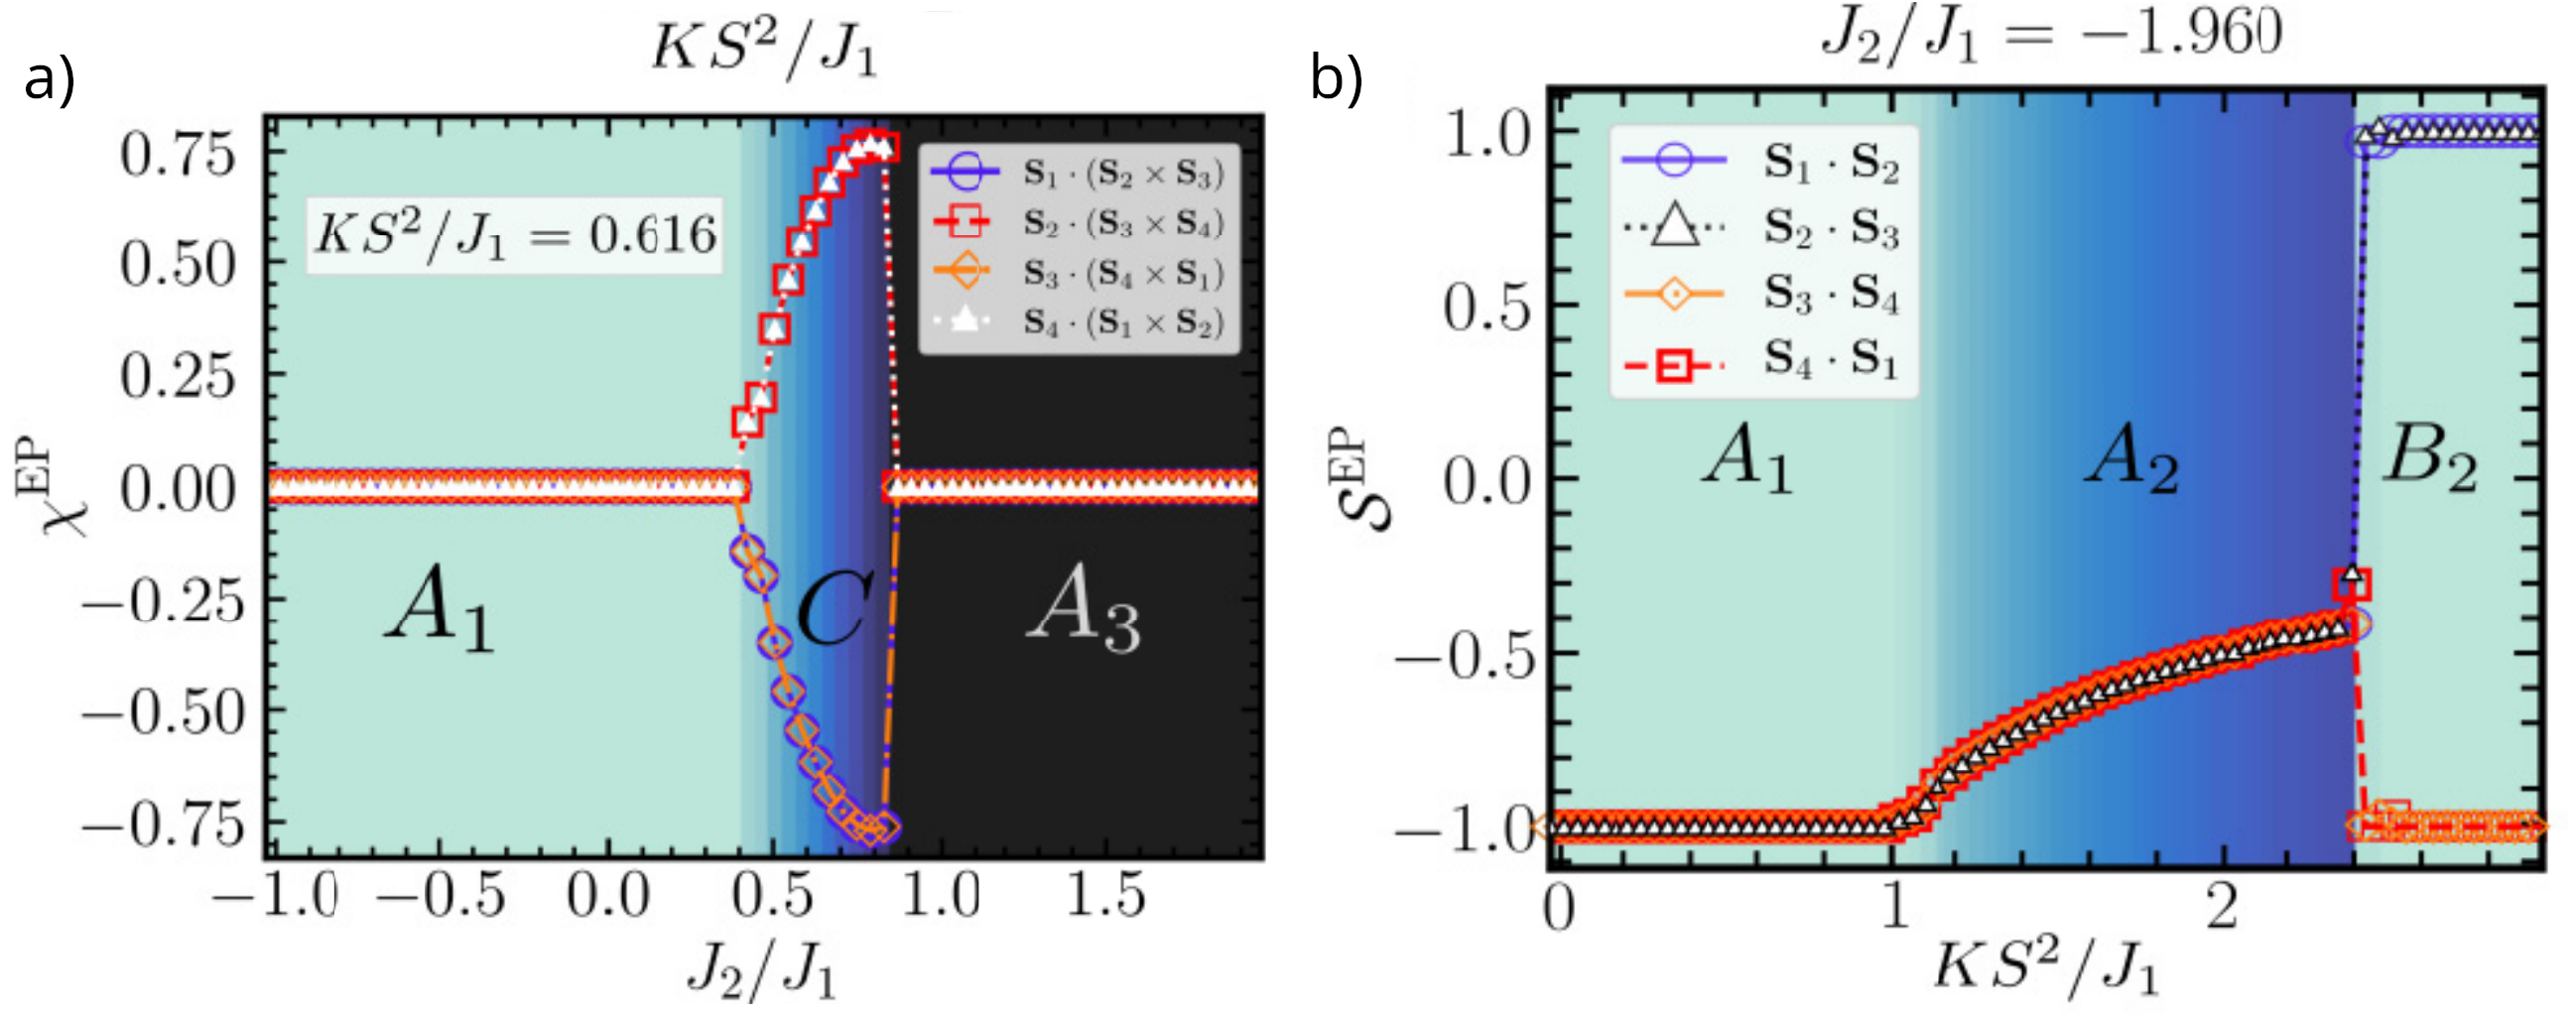
\includegraphics[width=0.8\linewidth]{figures/classical_transitions_combined}
    \caption{Scalar spin chiralities $\chiEP$ (a) and nearest-neighbor spin products $\SEP$ (b)
    along one-dimensional cuts through the phase diagram; the chirality grows
    continuously at the second-order transition from $A_1$ to $C$. Adapted from
    Ref.~\cite{Sobral2025}.}
    \label{fig:classical_transitions}
\end{figure}
The symmetry content of this pattern is the central observation. $\chiEP$ is
odd under time reversal alone, since every chirality flips sign. It is also odd
under $C_{4z}$ alone, since a rotation by $90^\circ$ maps the pattern
$(-1,1,-1,1)$ to $(1,-1,1,-1)$. The combined operation $\Theta C_{4z}$,
however, leaves the pattern invariant. This is precisely the defining symmetry
structure of an altermagnet, only that it now lives in the chirality channel
instead of the spin channel. The name orbital altermagnet comes from the fact
that in an electronic system a scalar spin chirality on a plaquette induces
circulating orbital currents. The associated orbital moments are finite locally
but cancel globally, again due to $\Theta C_{4z}$ rather than translation
\cite{Sobral2025}. Phase $C$ is the phase we will quantum-melt, and everything
that follows is the story of what survives.

\section{Quantum spin liquids and Schwinger bosons}
\label{sec:qsl}

\subsection{What is a quantum spin liquid?}
\label{sec:qsldef}

What do we mean when we say we quantum-melt an ordered phase into a quantum
spin liquid (QSL)? A QSL is not simply a magnet without order; it is something
more specific \cite{Savary2017}. Three properties characterize it. First, there
is no static magnetic order: $\langle \hat{\vS}_i \rangle = 0$ on every site,
even at $T = 0$. Second, the ground state is long-range entangled: it cannot be
adiabatically deformed into any product state, which is what separates a QSL
from a trivial paramagnet. Third, and most importantly, a QSL supports
fractionalized excitations, spin-$\tfrac{1}{2}$ spinons that cannot be created
by any single local operator, accompanied by emergent gauge fields.

A useful mental picture is Anderson's resonating valence bond (RVB) state
\cite{Anderson1973}: a superposition of all possible pairings of the spins into
singlets. No single pairing dominates, so the state has no spin order by
construction, and one can also see that it cannot be written as a product state
over any finite region. Breaking one singlet does not create a local spin flip
but two unpaired spin-$\tfrac{1}{2}$ objects that can move apart independently;
these are the spinons. We emphasize that spinons are not magnons. Magnons are
the spin-1 Goldstone modes of a broken-symmetry state, whereas spinons exist
precisely because no spin symmetry is broken.

The emergent gauge fields can be made more precise \cite{Savary2017}. Any
fractionalized description of a spin comes with a local constraint, and this
constraint structure generates a local gauge redundancy; the QSL corresponds to
a deconfined phase of the resulting emergent gauge theory. Which gauge
structure emerges matters for stability. In two spatial dimensions a compact
U(1) gauge theory with gapped matter is generically confining, so a U(1) spin
liquid is unstable, whereas a $\mathbb{Z}_2$ gauge theory possesses a stable
deconfined phase with topological order. We will meet exactly this distinction
below.

\subsection{The Schwinger boson representation}
\label{sec:sb}

How do we actually construct a spin liquid? The answer used in
Ref.~\cite{Sobral2025} is the Schwinger boson representation
\cite{Auerbach1994}. Every spin operator is rewritten in terms of two bosons,
\begin{equation}
    \label{eq:sbrep}
    \hat{\vS}_i = \frac{1}{2} \sum_{\sigma,\sigma'}
    \hat{b}^\dagger_{i\sigma}\, \boldsymbol{\sigma}_{\sigma\sigma'}\,
    \hat{b}_{i\sigma'},
    \qquad
    \hat{n}_i = \sum_{\sigma} \hat{b}^\dagger_{i\sigma} \hat{b}_{i\sigma} = 2S,
\end{equation}
where $\boldsymbol{\sigma}$ is the vector of Pauli matrices and $\sigma =
\uparrow, \downarrow$ labels the boson flavor. This rewriting is exact; it
embeds the spin Hilbert space into a larger bosonic one, and the local
constraint $\hat{n}_i = 2S$ projects back onto the physical subspace. The price
is a local U(1) gauge redundancy: the transformation $\hat{b}_{j\sigma} \to
e^{i\phi_j} \hat{b}_{j\sigma}$ with arbitrary site-dependent phases $\phi_j$
leaves all spin operators unchanged. The bosons carry spin $\tfrac{1}{2}$; they
are the spinons of the previous subsection.

Inserting this representation into \cref{eq:model} produces quartic boson
interactions. These are decoupled by a mean-field Hubbard-Stratonovich
transformation that introduces two complex bond fields with a transparent
physical meaning. The singlet amplitude $A_{ij}$ is the amplitude to create or
annihilate a spin-0 singlet pair on the bond $(i,j)$: one boson with spin up on
site $i$ and one with spin down on site $j$, combined antisymmetrically. It is
Anderson's valence bond made explicit. The hopping amplitude $B_{ij}$ is the
amplitude for a boson to hop from site $j$ to site $i$ while preserving its
spin, in analogy to tight-binding band theory. The decoupling yields the free
boson Hamiltonian
\begin{equation}
    \label{eq:hb}
    H_b = \frac{1}{2} \sum_{i,j} \sum_{\sigma}
    \left( B^{*}_{ij}\, \hat{b}_{i\sigma} \hat{b}^\dagger_{j\sigma}
    - \sigma A^{*}_{ij}\, \hat{b}_{i\sigma} \hat{b}_{j,-\sigma}
    + \mathrm{H.c.} \right)
    - \mu \sum_i \hat{n}_i,
\end{equation}
with $\sigma = \pm 1$ in the second term and a Lagrange multiplier $\mu$ that
enforces the constraint on average. A Fourier transformation followed by a
Bogoliubov transformation diagonalizes \cref{eq:hb} and yields the bosonic
quasiparticle bands. The pattern of the parameters $\{A_{ij}, B_{ij}\}$ on the
lattice, called the Ansatz, is what defines a particular spin liquid. Since a
self-consistent mean-field determination of these parameters is typically not
quantitatively reliable, Ref.~\cite{Sobral2025} instead studies the possible
Ansätze systematically; we come back to this strategy in \cref{sec:nearby}.

\subsection{Magnetic order, spin liquids, and the invariant gauge group}
\label{sec:igg}

The connection between the ordered phases and the spin liquids is made by the
bosonic band structure. The multiplier $\mu$ fixes the average boson density
$\langle \hat{n}_i \rangle = 2S$, and tuning $\mu$ and the couplings changes
the dispersion of the lowest band. Two situations can occur. If the lowest mode
reaches zero energy, the bosons condense at some momentum, and the condensate
wavefunction reconstructs exactly one of the classical spin textures of
\cref{sec:classical}. That is magnetic order. If instead the band stays gapped,
the bosons do not condense and the spins do not order. The very same Ansatz
then describes a fractionalized, long-range entangled state: the neighboring
spin liquid of that magnetic phase. This is the bridge between the altermagnet
and the concept of a QSL.

Not all spin liquids obtained in this way are of the same type. The type is
determined by the invariant gauge group (IGG), the subgroup of the U(1) gauge
transformations that leaves the Ansatz invariant. If a continuous U(1) subgroup
survives, the result is a U(1) spin liquid, which, as discussed in
\cref{sec:qsldef}, is generically unstable in two dimensions. If only the sign
flip $\hat{b}_i \to -\hat{b}_i$ survives, the result is a $\mathbb{Z}_2$ spin
liquid, a stable topological phase. In practice, adding imaginary $B_{ij}$ to
an Ansatz generically reduces the IGG from U(1) to $\mathbb{Z}_2$, because
imaginary bonds are sensitive to phase transformations that real bonds are not.
The IGG therefore determines the physical nature of the spin liquid's
excitations and its stability.

\section{Nearby spin liquids}
\label{sec:nearby}

\subsection{Matching phases to Ansätze}
\label{sec:matching}

The strategy to find the neighboring spin liquid of each classical phase is to
reverse-engineer the Ansatz \cite{Sobral2025}:
\begin{enumerate}
    \item Choose a pattern of $A_{ij}$ and $B_{ij}$ on nearest-neighbor and
          next-nearest-neighbor bonds.
    \item Diagonalize the free boson Hamiltonian \eqref{eq:hb} and find the
          lowest mode.
    \item Tune $\mu$ such that this mode condenses.
    \item Reconstruct the spin texture from the condensate and check whether it
          matches one of the phases of \cref{tab:phases}.
\end{enumerate}
The minimal Ansatz whose condensation reproduces a given phase is the natural
candidate, and its gapped regime is the neighboring QSL, which inherits the IGG
and the discrete symmetries of the parent phase. It turns out that
nearest-neighbor and next-nearest-neighbor bonds are sufficient for all six
phases, without any enlargement of the unit cell.

\begin{figure}[th]
    \centering
    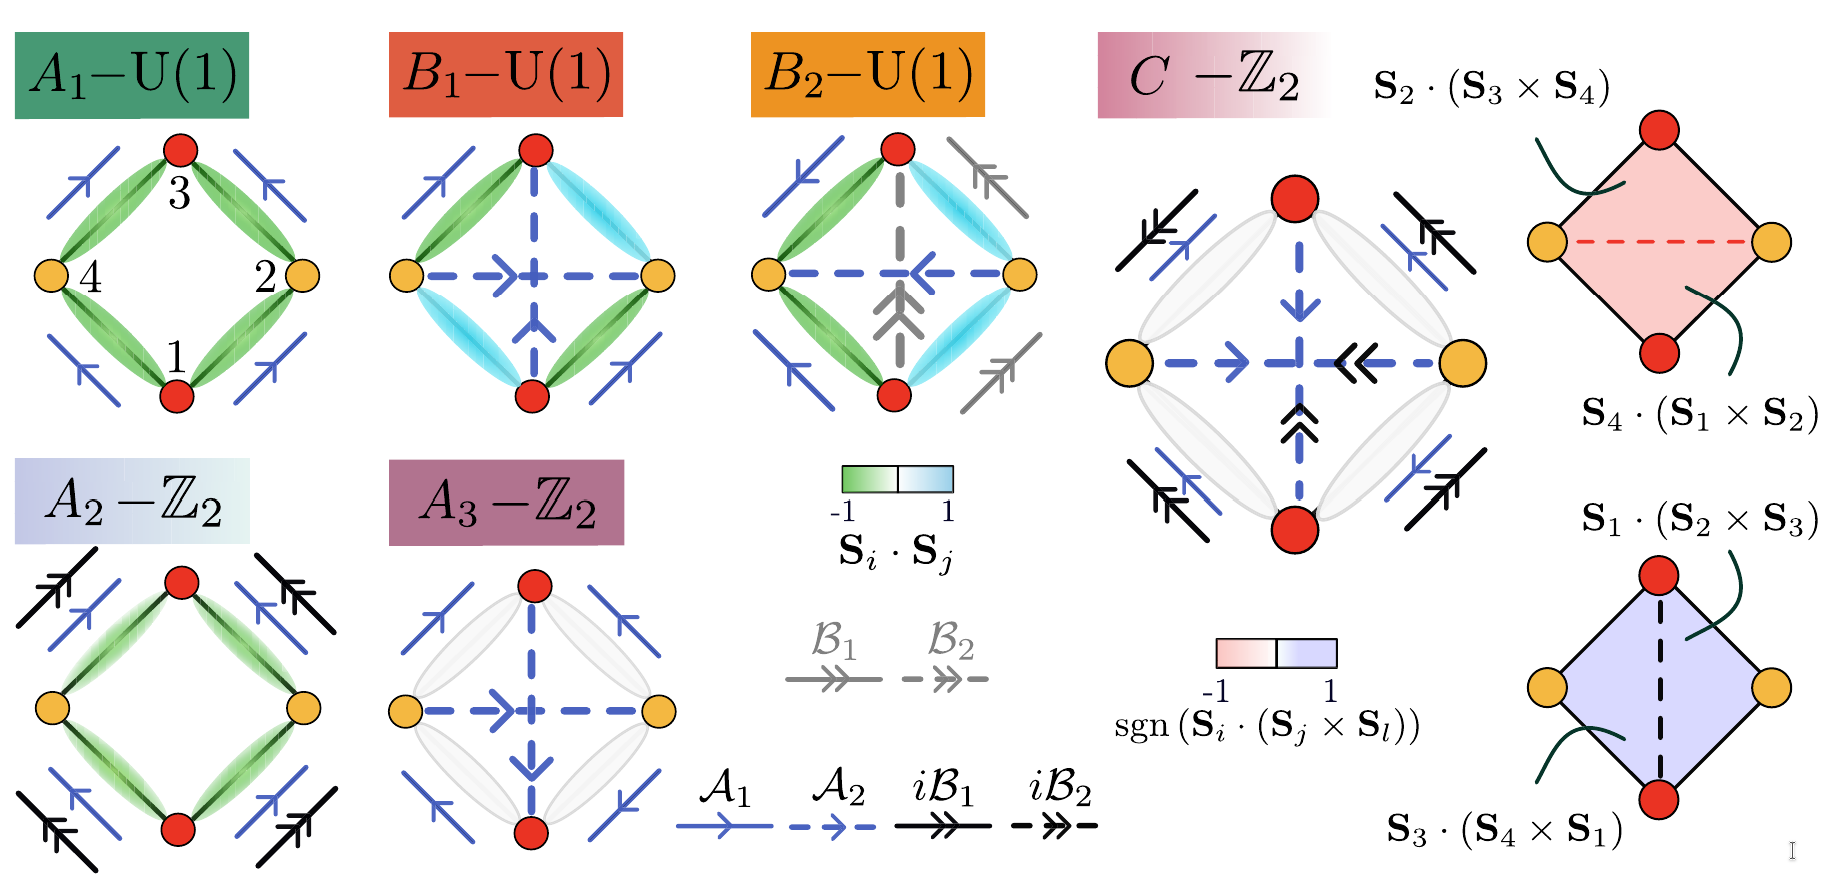
\includegraphics[width=0.9\linewidth]{figures/schwinger_boson_ansätze}
    \caption{Schwinger boson Ansätze associated with the six magnetic phases of
    \cref{tab:phases}. Blue arrows denote real singlet amplitudes $A_{ij}$,
    black and gray arrows denote real and imaginary hopping amplitudes
    $B_{ij}$. The colored ellipses show the correlators $\langle \SEP \rangle$
    evaluated in the gapped spin-liquid regime; for the Ansatz of phase $C$ the
    staggered chirality pattern $\langle \chiEP \rangle$ is nonzero as well.
    Adapted from Ref.~\cite{Sobral2025}.}
    \label{fig:ansaetze}
\end{figure}

\Cref{fig:ansaetze} shows the resulting Ansätze. On top of each Ansatz the
correlators $\langle \SEP \rangle$ are drawn as colored ellipses, evaluated
directly in the gapped spin-liquid regime, that is, without any condensation.
One can therefore read off the spatial symmetry of each spin liquid without
ever returning to the ordered phase. The result confirms the symmetry
inheritance. The spin liquids of $A_1$, $A_2$, and $A_3$ have isotropic
$\langle \SEP \rangle$ and are fully symmetric, while the spin liquids of $B_1$
and $B_2$ show exactly the nematic patterns of their parent phases; in all five
cases $\langle \chiEP \rangle = 0$. The gauge groups are listed in
\cref{tab:phases}: the Ansätze of $A_1$, $B_1$, and $B_2$ give U(1) spin
liquids, while those of $A_2$, $A_3$, and $C$ involve imaginary $B_{ij}$ or
further-neighbor bonds and give $\mathbb{Z}_2$ spin liquids.

\subsection{The altermagnetic spin liquid}
\label{sec:amsl}

The spin liquid associated with phase $C$ is the main result. Its Ansatz is the
only one that shows a nonzero chirality pattern in the spin-liquid regime, and
its IGG is $\mathbb{Z}_2$. In the gapped regime the bosons are not condensed,
so $\langle \hat{\vS}_i \rangle = 0$ everywhere and spin-rotation invariance is
fully restored. The correlators tell us what remains. The spin products are
isotropic, so $C_{4z}$ is intact in the spin sector. The chirality correlator,
however, stays staggered, $\langle \chiEP \rangle \propto (-1,1,-1,1)$: time
reversal remains broken in spin-rotation-invariant observables, with exactly
the $\Theta C_{4z}$ pattern of the orbital altermagnet.

Let us state this clearly. There is no spin order anywhere in this phase, and
yet the altermagnetic arrangement of scalar chiralities survives. The phase
combines $\mathbb{Z}_2$ topological order with a persistent altermagnetic
chirality pattern and is therefore called the altermagnetic spin liquid
\cite{Sobral2025}. It is a symmetry-enriched topological phase that was first
described in this work. The altermagnetic character outlives the spin order
that originally defined it.

Being a $\mathbb{Z}_2$ spin liquid, the phase also hosts vison excitations,
gapped vortices of the emergent gauge field. In the altermagnetic spin liquid
they are associated with local distortions of the chirality pattern, which
makes them a natural target for local experimental probes
\cite{Sobral2025,Jahin2025}.

\section{Conclusion and outlook}
\label{sec:conclusion}

Three points summarize this report. First, the checkerboard $J_1$-$J_2$-$K$
model hosts, besides collinear and nematic phases, a noncoplanar orbital
altermagnet, phase $C$, whose staggered scalar chirality pattern is invariant
under the combined operation $\Theta C_{4z}$. Second, within the Schwinger
boson construction every classical phase has a neighboring quantum spin liquid,
and the discrete symmetries of the parent phase are inherited by the spin
liquid, visible in the correlators $\langle \SEP \rangle$ and $\langle \chiEP
\rangle$. Third, the neighbor of the orbital altermagnet is the altermagnetic
$\mathbb{Z}_2$ spin liquid: a phase without any spin order that nevertheless
carries a persistent altermagnetic chirality pattern together with topological
order.

On the experimental side, the most direct route to this physics would be local
probes that are sensitive to bond chiralities, for example scanning tunneling
microscopy or local susceptibility measurements, which could also detect the
vison excitations of the $\mathbb{Z}_2$ phase \cite{Jahin2025}. The open
question is whether candidate materials exist. Frustrated altermagnets are
largely unexplored, but the experimental indications in Mn$_5$Si$_3$
\cite{Biniskos2022,Surgers2024} and CsCr$_3$Sb$_5$ \cite{Xu2025} suggest that
the interplay of altermagnetism and frustration is realized in real compounds.
The framework presented here also extends naturally to doped systems, where the
fractionalized phases lead to spin-split Fermi surfaces without any breaking of
spin-rotation symmetry; this is discussed in Ref.~\cite{Sobral2025} and lies
beyond the scope of this report. The paper lays the foundation for the study of
altermagnetic quantum spin liquids and opens the map of frustrated
altermagnets.

\printbibliography

\end{document}
